\documentclass[10pt]{ctexbeamer}

\usepackage{bm}
\usepackage{tikz}
\usepackage{amsmath}
\usepackage{graphicx}
\usepackage{gensymb}
\usepackage{hyperref}

\usetheme[color blocks]{Verona}
\usefonttheme[onlymath]{serif}% 数学公式字体设置

\author{Norsesun}
\date{最后更新:\today}
\logo{
\includegraphics[height=1.2cm]{../Pngtree owl double exposure.png}}
\title{第一章的复习}
\subtitle{Review of Chapter 1}

% \definecolor{airforceblue}{rgb}{.36,.54,.66}
% \setbeamercolor{background canvas}{bg=airforceblue}
\AtBeginSubsection[circle, subsections numbered]
{
	\begin{frame}{要点目录}
		\tableofcontents[currentsubsection]
	\end{frame}
}

\begin{document}
    \frame{\titlepage}
    \section{地球和地球仪}
    \subsection{地球的形状大小}
    \begin{frame}{地球的形状大小}{地球并不是一个正球体,而是一个两极稍扁、赤道略鼓的不规则球体}
    \begin{figure}
        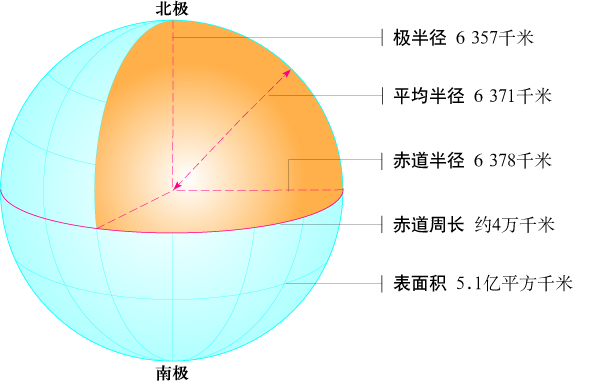
\includegraphics[width=.79\textwidth]{assets/earth shape.jpg}
    \end{figure}
    \structure{平均半径$6371km$, 最大周长$40000km$, 表面积$5.1\times10^{12} km^2$ }
    \end{frame}

    \begin{frame}{地球仪(Globe)}{地轴(Earth's Axis)相对于地球公转轨道面是倾斜的}
        \begin{columns}
            \column{0.5\textwidth}
            \only<1>{
                
\includegraphics[width=.99\textwidth]{assets/earth little.jpg}
            }
            \only<2>{
                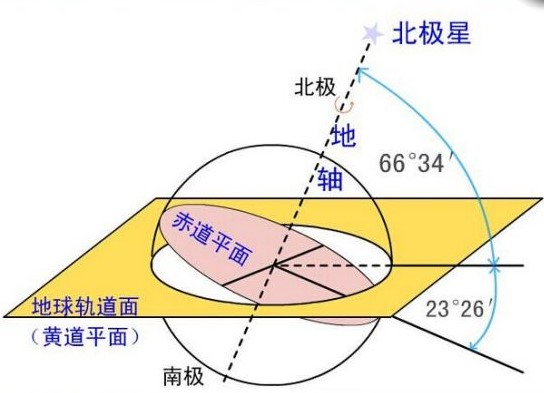
\includegraphics[width=.99\textwidth]{assets/earth axis.jpg}
            }
            \column{0.47\textwidth}
            \begin{description}
                \item[地轴] 人们假想的轴,与黄道面约成 $66.5\degree$角。\\
                \item[两极] 地轴与地球表面相交的两点,其中对着北极星方向的点叫\alert{北极(North Pole)},与之对应的点是南极(South Pole)。
            \end{description}
        \end{columns}
    \end{frame}

    \subsection{经线与纬线}
    \begin{frame}{地球仪上的点与线}
        \begin{columns}
            \column{0.50\textwidth}
            \begin{figure}
                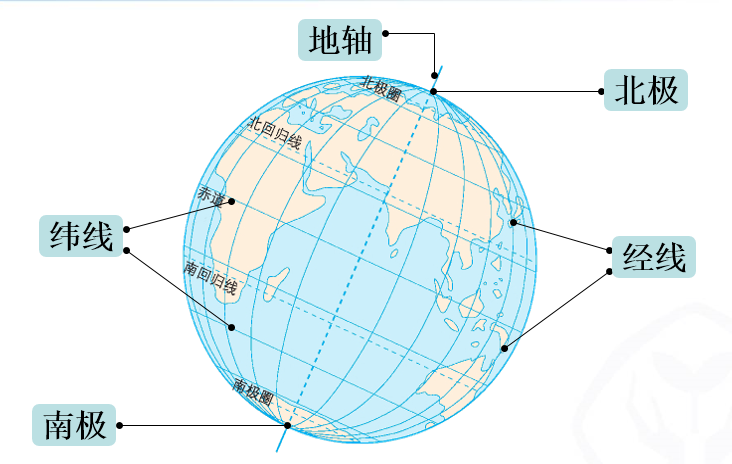
\includegraphics[width=.99\textwidth]{assets/little earth.png}
            \end{figure}
            \begin{figure}[c]
                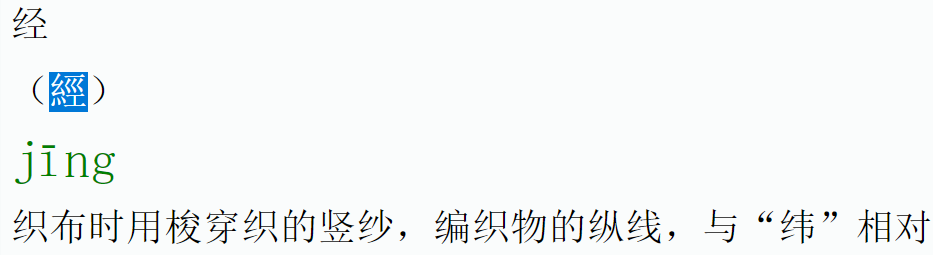
\includegraphics[width=.89\textwidth]{assets/jing.png}
                \caption{在"上北下南,左西右东"的情况下,\alert{经线是竖着的}}
            \end{figure}
            
            \column{0.50\textwidth}
            \begin{description}
                \item[赤道] 与南北极距离相等的大圆圈,叫赤道(Equator)。\\
                \item[纬线] 所有与赤道平行的\alert{圆圈}叫纬线(Parallel)。赤道是最大的纬线圈。纬线指示东西。\\
                \item[经线] 连接南北两极并垂直于纬线的线(\alert{半圆}),也叫\alert{子午线(Meridian Line)}。经线指示南北。
            \end{description}
        \end{columns}
    \end{frame}

    \begin{frame}{纬度(Latitude)}
        \begin{columns}
            \column{0.50\textwidth}
            \begin{description}
                \item[纬度] \alert{赤道的纬度是$0\degree$},向南向北各$90\degree$,分别用$N$ 和 $S$表示。\\
                \item[高中低纬度] 全球 $0\degree - 30\degree$为低纬度地区,$30\degree - 60\degree$为中纬度地区。
                    $60\degree - 90\degree$为高纬度地区\\
                \item[南北半球] \alert{赤道划分南北半球},赤道往北是北半球,往南是南半球。
            \end{description}
            \column{0.50\textwidth}
            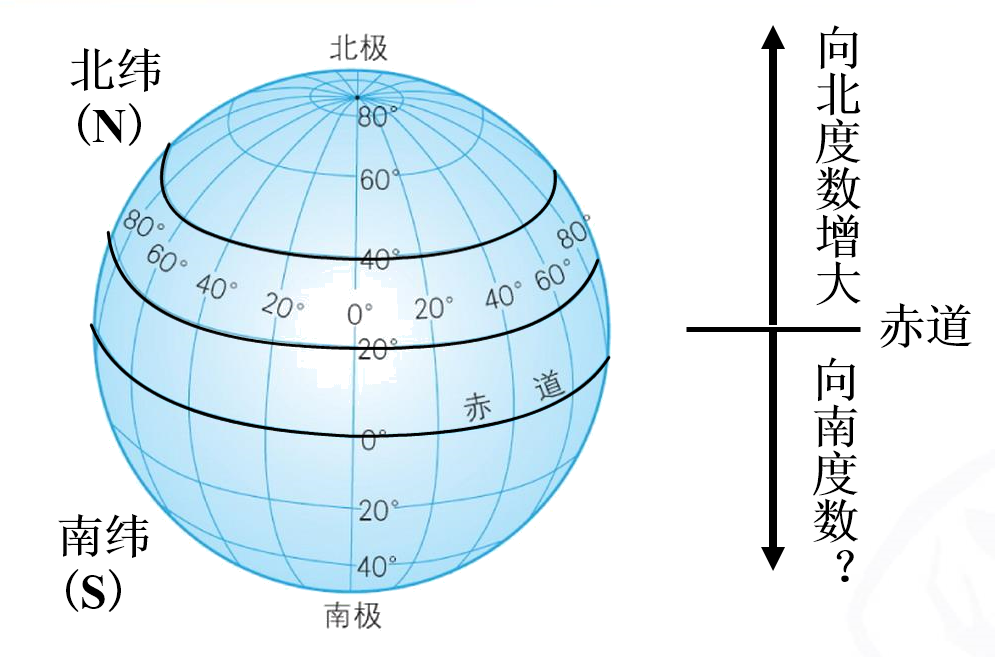
\includegraphics[width=.99\textwidth]{assets/latitude.png}
        \end{columns}
    \end{frame}

    \begin{frame}{经度(Longitude)}
        \begin{columns}
            \column{0.50\textwidth}
            \begin{description}
                \item[经度] \alert{本初子午线的经度是$0\degree$},向东向西各$180\degree$,分别用$E$ 和 $W$表示。\\
                \item[经度的特征] 东经和西经的$180\degree$是重合的,通常把它称为$180\degree$经线。任意
                    两条相对的经线(加起来是$180\degree$,而且刚好一个东经一个西经)组成一个经线圈。\\
                \item[东西半球] \alert{$20\degree W$和$160\degree E$组成的经线圈划分东西半球},$20\degree W$往东是东半球,$20\degree W$往西是西半球。
            \end{description}
            \column{0.50\textwidth}
            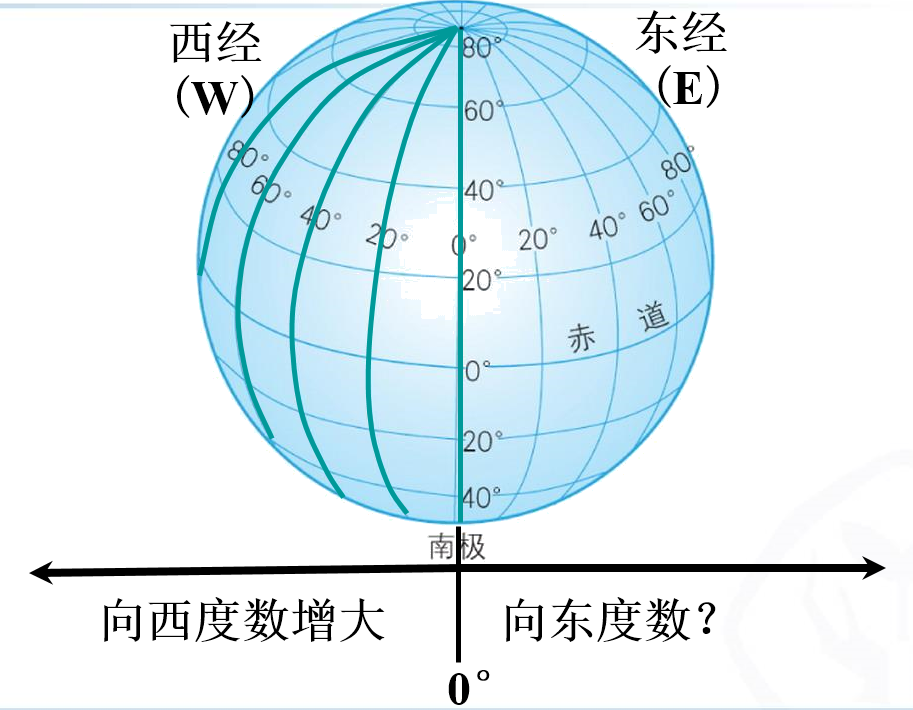
\includegraphics[width=.99\textwidth]{assets/longitude.png}
        \end{columns}
        
    \end{frame}
    \begin{frame}{问题1}{知识点:半球的划分}
        \begin{columns}
            \column{0.49\textwidth}
            \begin{block}{}
                北纬一定在北半球,南纬一定在南半球吗?\\
                东经一定在东半球,西经一定在西半球吗?
            \end{block}
            \column{0.49\textwidth}
            \begin{figure}
                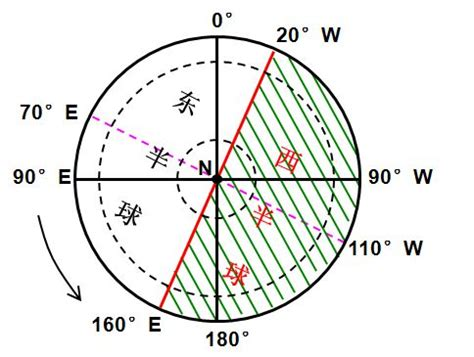
\includegraphics[width=0.89\textwidth]{assets/line 2.jpg}
                \caption{从北极上空俯视地球}
            \end{figure}
            
        \end{columns}
        \only<2>{
            北纬一定在北半球,南纬一定在南半球。\\
            因为南北半球的分界线是赤道($0\degree$纬线)。\\
            东经不一定在东半球,西经不一定在西半球。\\
            因为东西半球的分界线
            不是本初子午线($0\degree$)和$180\degree$经线组成的经线圈,\\
            而是\alert{$20\degree W$和$160\degree E$组成的经线圈}。
        }
    \end{frame}

    \begin{frame}{问题2}{知识点:学会画图思考解决问题}
        \begin{columns}
            \column{0.49\textwidth}
            \begin{block}{}
                $0\degree$经线往东是东经还是西经?\\
                $180\degree$经线往东是东经还是西经?\\
                $20\degree W$往东是东半球还是西半球?\\
                $160\degree E$往东是东半球还是西半球?\\
            \end{block}
            \column{0.49\textwidth}
            \begin{figure}
                \pause
                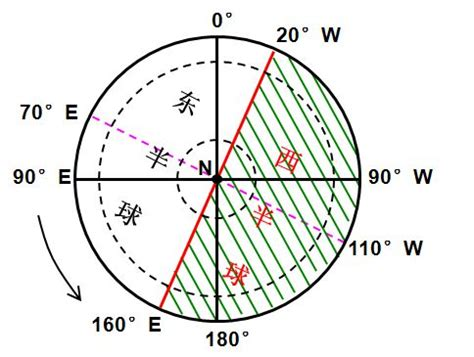
\includegraphics[width=0.89\textwidth]{assets/line 2.jpg}
                \caption{从北极上空俯视地球}
            \end{figure}
            
        \end{columns}
        \only<2>{
            $0\degree$经线往东是东经,$180\degree$经线往东是西经。\\
            $20\degree W$往东是东半球,$160\degree E$往东是西半球。

        }
    \end{frame}

    \begin{frame}[fragile]{利用经纬网定位}{利用经纬网可以确定地球表面某一点的位置}
        \begin{columns}
            \column{0.49\textwidth}
            黄桥镇的经纬度约为:$(27\degree N, 111\degree E)$。\\
            \vspace{2em}
            \alert{伦敦(London)}的经纬度: $(51\degree N, 0\degree)$。科学家们以穿过
                格林尼治天文台(Greenwich Observatory)旧址的经线作为起始经线,即$0\degree$经线。
                这个天文台正是位于伦敦。

                \begin{block}{3D 地球(384318-parabola2020)}
                    \url{http://www.tuxingis.com/wish3dearth.html}\\
                    \url{http://online.wish3d.com/Wish3DEarth/manage/index.html#//online.wish3d.com/Wish3DEarth/manage/sceneList.html}
                \end{block}
            \column{0.49\textwidth}
            \begin{figure}
                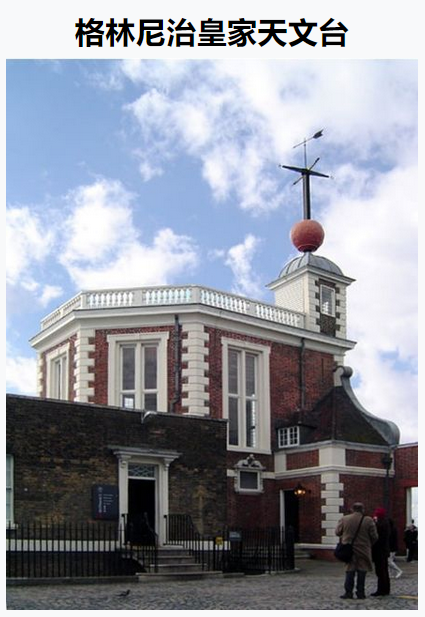
\includegraphics[width=0.79\textwidth]{assets/royal ovservatory Greenwich.png}
            \end{figure}
        \end{columns}
    \end{frame}

    \begin{frame}[plain, noframenumbering, label=Question]
        \begin{center}
            \Huge{你get到了吗?}
        \end{center}
        \begin{figure}
            
\includegraphics[width=0.2\textwidth]{../jie/wha.jpg}
        \end{figure}
    \end{frame}
\end{document}
